\documentclass{article}

\title{Zumobot case study}
\date{29.6.2017}
\author{Javier Reyes}

\usepackage{graphicx}
\usepackage{booktabs}
\usepackage{amsmath}

\usepackage[backend=biber, style=ieee]{biblatex}
\bibliography{report}


\begin{document}

\maketitle
\pagenumbering{gobble}
\newpage
\pagenumbering{arabic}

\tableofcontents
\newpage

\section*{Introduction}

One of the most used study cases in Control Theory is the Inverted Pendulum analysis, as it present an unstable open-loop characteristic but is also possible to stabilize on a closed-loop configuration.

Here we present the anyalis of the Zumobot 32U4, a small robot available on the market. It is equiped with two DC motors, an Arduino-based board with several periferials.

TODO: Complete

\section{System analysis}

An inverted pendulum can be represented as a cart moving on an horizontal axis, connected to a rigid body pendulum.

\begin{figure}[h!]
	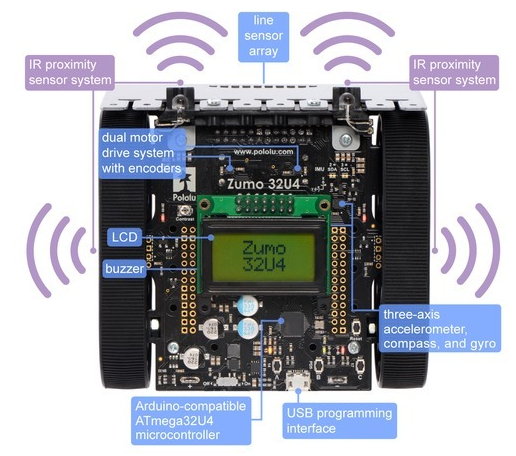
\includegraphics{img/zumo-superior.png}
	\centering
	\caption{Superior view of the zumo robot.}
	\label{fig:sup-zumo}
\end{figure}

The figure \ref{fig:sup-zumo} shows the robot that will be modeled as a Wheeled Inverted Pendulum.

\begin{table}[h!]
	\centering
	\caption{Basic table.}
	\label{tab:tab1}
	\begin{tabular}{ccc}

		\toprule

		header A & header B & header C\\

		\midrule

		a & b & c\\
		c & d & e\\
		f & g & h\\

		\bottomrule

	\end{tabular}
\end{table}

Text of the section\footnote{\label{fn1}This is a footnote}.

Text of the section after the footnote \ref{fn1}.

TODO: Complete

\section{Mathematical development}

Through the literature is possible to find several approaches to obtain a model for the IP.

To fully model the dynamic behavior of the zumo robot, we need to consider the equations that govern the movement as rigid body.

\subsection{First approach - Sum of forces}

The first approach considered here is described in \cite{SUL03}, as follows:

The equations of motion are obtained from the sum of forces in the cart for the horizontal direction.

\begin{equation} \label{sfch}
F-b\dot{x}-N=M\ddot{x}
\end{equation}

Now considering the pendulum itself, the force applied in the horizontal direction due to the momentum of the pendulum is determined as:

\begin{equation} \label{dhfp}
\tau=r\cdot F=I\cdot \ddot{\theta}
\end{equation}

Given the fact that the moment of inertia of a pendulum of mass $m$ is defined as $I=m\cdot L^2$, the previous equation can be rewritten as:

\begin{equation} \label{dhfp2}
F=\frac{I\cdot \ddot{\theta}}{r}=\frac{m\cdot l^2\cdot \ddot{\theta}}{l}=m\cdot l\cdot \ddot{\theta}
\end{equation}

Obtaining the component of the force prevoiusly defined in the horizontal direction:

\begin{equation} \label{sfph}
F=m\cdot l\cdot \ddot{\theta}\cdot \cos{\theta}
\end{equation}

Now, the component of the centripetal force acting on the pendulum is similar to the one in \ref{dhfp2}, but the horizontal component of this force is:

\begin{equation} \label{scfph}
F=m\cdot l\cdot \ddot{\theta}\cdot \sin{\theta}
\end{equation}

Summing the previously defined forces present in the horizontal direction, we obtain the following expression:

\begin{equation} \label{scfph}
F=m\cdot l\cdot \ddot{\theta}\cdot \sin{\theta}
\end{equation}

\section{System model}

Text of the section.

\section{Regulator}

Text of the section.

\section{Implementation}

Text of the section.

\begin{appendix}
	\newpage
	\listoffigures
	\newpage
	\listoftables
\end{appendix}

\newpage
\printbibliography

\end{document}
